\documentclass[14pt,aspectratio=1610]{beamer}
%\documentclass[12pt,aspectratio=1610,handout]{beamer}
\usepackage{csu-theme}
\usepackage{arrays}
\usepackage{booktabs}
\usetikzlibrary{shapes.misc, backgrounds}
\usetikzlibrary{calc}

\tikzset{
  hashBucket/.style = {
    draw,
    rounded rectangle,
    align=center,
    anchor=west,
    font=\small,
    very thick,
    fill=CSUslate
  },
  chain bucket/.style = {
    draw,
    fill=CSUslate,
    very thick,
    rounded corners=2pt,
  },
  chain element/.style = {
    node of array,
    minimum height=8.5mm,
    fill=CSUcyan,
    text depth=.2ex
  }
}


\title{\Huge{}Hashing \& Hash Tables \\with Open Addressing}
\subtitle{CSCI 315: Data Structure Analysis\\Chapter 5 of \href{https://opendatastructures.org/ods-cpp.pdf}{Open Data Structures}}
%\author{Sean T. Hayes, Ph.D.}
\institute{Charleston Southern University}

%% Comment out date to use default (today)
% \date{March 27, 2025}
\subject{Software Programming}
%\keywords{}

\setlength{\parskip}{0.5em}

\graphicspath{{../imgs/}{../imgs/hashtables}}

\begin{document}

\begin{frame}
  \titlepage
\end{frame}

\section*{Review}

\begin{frame}{Maps/Dictionary}
Map (dictionary) is a relation between a set of keys\\
and set of values.

\begin{figure}
\centering

\includegraphics[width=0.667\textwidth]{maping-keys-values}
\end{figure}
\end{frame}


\begin{frame}{Implementing Dynamic Maps/Dictionaries}

\begin{itemize}
\item
  We want a data structure in which finds/searches are very fast.
  \begin{itemize}
  \item
    As close to $O(1)$ as possible.
  \item
    With the minimum number of executed instructions per method.
  \end{itemize}
\item
  Insert and Deletes should be fast too.
\item
  Objects in a map have unique keys. A key may be:
  \begin{itemize}
  \item
    A single property/attribute value, or
  \item
    Created from multiple properties/values.
  \end{itemize}
\end{itemize}
\end{frame}

\begin{frame}{A Conceptual View of Hash Tables}
  \begin{figure}
  \centering
    \begin{tikzpicture}[node of array/.append style={minimum height=8mm,fill=CSUgold}]
      \ArrayLabel{Table}
      \ArrayNodeVertical{}
      \fill (val) circle(2pt);
      \node[block] (firstEl) [fit=(val)]{};

      \ArrayNodeVertical{}
      \fill (val) circle(2pt);
      \coordinate (ptr) at (val);
      \node[chain element, anchor=west, name=key] at ([xshift=2cm, yshift=8mm] prev.east) {key = 1};
      \node[chain element, anchor=west, name=valval] at ([xshift=-1pt] key.east) {val5};
      \begin{scope}[on background layer]
        \node[chain bucket, fit=(key) (valval)] (bucket) {};
        % \node[chain bucket] (bucket) [fit=(key) (valval)]{};
      \end{scope}
      \draw[link] (ptr) -- (bucket);
      \node[anchor=south] at(bucket.north) {Buckets};

      \ArrayNodeVertical{}
      \fill (val) circle(2pt);
      \coordinate (ptr) at (val);
      \node[chain element, anchor=west, name=key] at ([xshift=2cm] prev.east) {key = 2};
      \node[chain element, anchor=west, name=valval] at ([xshift=-1pt] key.east) {val4};
      \begin{scope}[on background layer]
        \node[chain bucket,fit=(key) (valval)] (bucket) {};
      \end{scope}
      \draw[link] (ptr) -- (bucket);


      \ArrayNodeVertical{}
      \fill (val) circle(2pt);

      \ArrayNodeVertical{}
      \fill (val) circle(2pt);
      \coordinate (ptr) at (val);
      \node[chain element, anchor=west, name=key] at ([xshift=2cm] prev.east) {key = 4};
      \node[chain element, anchor=west, name=valval] at ([xshift=-1pt] key.east) {val3};

      \node[chain element, anchor=west, name=key2] at ([xshift=5pt] valval.east) {key = 28};
      \node[chain element, anchor=west, name=valval2] at ([xshift=-1pt] key2.east) {val2};

      \begin{scope}[on background layer]
        \node[chain bucket,fit=(key) (valval) (key2) (valval2)] (bucket) {};
      \end{scope}
      \draw[link] (ptr) -- (bucket);

      \ArrayNodeVertical{}
      \fill (val) circle(2pt);

      \ArrayNodeVertical{}
      \fill (val) circle(2pt);

      \ArrayNodeVertical{}
      \fill (val) circle(2pt);
      \coordinate (ptr) at (val);
      \node[chain element, anchor=west, name=key] at ([xshift=2cm] prev.east) {key = 15};
      \node[chain element, anchor=west, name=valval] at ([xshift=-1pt] key.east) {val1};
      \begin{scope}[on background layer]
        \node[chain bucket,fit=(key) (valval)] (bucket) {};
      \end{scope}
      \draw[link] (ptr) -- (bucket);


      \draw [decorate, decoration = {brace,raise=5pt,amplitude=8pt}, very thick] ([xshift=-1cm]prev.south west) -- ([xshift=-1cm]firstEl.north west) node [pos=0.5,left=12pt,anchor=south, rotate=90] {hash value / index};

    \end{tikzpicture}
  \end{figure}
\end{frame}

\begin{frame}{Generating Hash Codes}
  \begin{itemize}
    \item
      Note that the key may not be an integer that can neatly be used for hashing.\\
      For example,
      \begin{itemize}
        \item Floating-point numbers: (e.g., \texttt{3.14159}, \texttt{23543.43}, \texttt{3.997E-8})
        \item String values: (e.g., \texttt{"Alice"}, \texttt{"Dear diary"}, \texttt{":-)"})
        \item Objects of custom classes.
      \end{itemize}
    \item
      We need to make a hash-code function for each type we want to use as a key in our hash table.
  \end{itemize}
\end{frame}

\begin{frame}{Dealing with Collisions}
  A problem arises when we have two keys that hash in the same array entry --- this is called a \emph{collision}.
  
  \onslide<2->{There are two ways to resolve collision:}
  \begin{itemize}
    \item<3->
      \emph{Hashing with Chaining} (a.k.a., ``Separate Chaining''):\\
      Every hash-table entry contains a pointer to a linked list of keys that hash in the same entry.
    \item<4->
      \emph{Hashing with Open Addressing}:\\
      Every hash-table entry contains only one key. If a new key hashes to a filled table entry, systematically examine other table entries until you find one empty entry to place the new key.
  \end{itemize}
\end{frame}

\section{Open Addressing}

\begin{frame}{Hash Tables with Open Addressing}
  \centering{}
  %\centerline{%
    Insert where the key is
    \alt<-2>{%
      1.%
    }{%
      \alt<-4>{%
        2.%
      }{%
        \alt<-6>{%
          15.%
        }{%
          \alt<-8>{%
            28.%
          }{
            \alt<-10>{%
              4.%
            }{%
              5.%
            }%
          }%
        }%
      }%
    }\\%
  %}
  %
  \begin{tikzpicture}[%
    node of array/.append style={%
      minimum height=8mm,
      inner sep=0,
      text depth=.1ex,
      minimum width=12mm,
      %fill=CSUslate,
      %text=white!50!CSUslate
    },%
    subcomponent of array el/.append style={minimum width=18mm, node distance=-1.4pt},%
  ]%
    \ArrayLabel{}
    
      \begin{scope}[node of array/.append style = {fill=CSUslate, text=white!50!CSUslate}]
        \ArrayNodeVertical{?,?}
      \end{scope}
      \node[anchor=south, text depth=.2ex, name=keyCol] at ([yshift=-1pt] val.north) {key};
      \node[anchor=south, text depth=.2ex, name=keyCol] at ([yshift=-1pt] lastElValue.north) {value};
    
      \alt<1>{
        \begin{scope}[node of array/.append style = {fill=CSUslate, text=white!50!CSUslate}]
          \ArrayNodeVertical[]{?,?}
        \end{scope}
      }{
        \ArrayNodeVertical[]{1,Obj1}
      }
      \onslide<2->{\node[name=bucketIndex, anchor=west, text depth=.1ex] at ([xshift=3pt]lastElValue.east) {index is \texttt{1}};}

      \alt<-3>{
        \begin{scope}[node of array/.append style = {fill=CSUslate, text=white!50!CSUslate}]
          \ArrayNodeVertical[]{?,?}
        \end{scope}
      }{
        \ArrayNodeVertical[]{2,Obj2}
      }
      \onslide<4->{\node[name=bucketIndex, anchor=west, text depth=.1ex] at ([xshift=3pt]lastElValue.east) {index is \texttt{2}};}

      % Index 3
      \begin{scope}[node of array/.append style = {fill=CSUslate, text=white!50!CSUslate}]
        \ArrayNodeVertical{?,?}
      \end{scope}

      \node[rotate=90] at ([xshift=-1.5cm]val.south west) {hash index};

      % Index 4
      \alt<-7>{
        \begin{scope}[node of array/.append style = {fill=CSUslate, text=white!50!CSUslate}]
          \ArrayNodeVertical[]{?,?}
        \end{scope}
      }{
        \ArrayNodeVertical[]{28,Obj4}
      }
      \onslide<8->{\node[name=bucketIndex, anchor=west, text depth=.1ex] at ([xshift=3pt]lastElValue.east) {index is \texttt{4}};}

      % Index 5
      \alt<-9>{
        \begin{scope}[node of array/.append style = {fill=CSUslate, text=white!50!CSUslate}]
          \ArrayNodeVertical[]{?,?}
        \end{scope}
      }{
        \ArrayNodeVertical[]{4,Obj5}
      }
      \onslide<10->{\node[name=bucketIndex, anchor=west, text depth=.1ex] at ([xshift=3pt]lastElValue.east) {index is \texttt{4}};}

      % Index 6
      \alt<-11>{
        \begin{scope}[node of array/.append style = {fill=CSUslate, text=white!50!CSUslate}]
          \ArrayNodeVertical[]{?,?}
        \end{scope}
      }{
        \ArrayNodeVertical[]{5,Obj6}
      }
      \onslide<12->{\node[name=bucketIndex, anchor=west, text depth=.1ex] at ([xshift=3pt]lastElValue.east) {index is \texttt{5}};}

      % Index 7
      \alt<-5>{
        \begin{scope}[node of array/.append style = {fill=CSUslate, text=white!50!CSUslate}]
          \ArrayNodeVertical[]{?,?}
        \end{scope}
      }{
        \ArrayNodeVertical[]{15,Obj3}
      }
      \onslide<6->{\node[name=bucketIndex, anchor=west, text depth=.1ex] at ([xshift=3pt]lastElValue.east) {index is \texttt{7}};}
    
  \end{tikzpicture}
\end{frame}

% \begin{frame}{Hash Tables with Open Addressing}
% \centerline{%
% Insert where the key is 
% \alt<-2>{%
%   1.%
% }{%
%   \alt<-4>{%
%     2.%
%   }{%
%     \alt<-6>{%
%       15.%
%     }{%
%       \alt<-8>{%
%         28.%
%       }{
%         \alt<-10>{%
%           4.%
%         }{%
%           5.%
%         }%
%       }%
%     }%
%   }%
% }}
% \hspace{2cm}%
% \begin{tikzpicture}
%   \ArrayLabel{table}
%   \ArrayNodeVertical{}

%   \alt<1>{
%     \ArrayNodeVertical{}
%   }{
%     \ArrayNodeVertical[CSUgold]{}
%     \fill (valPtr) circle(2pt);
%     \node[hashBucket,name=bucket] at ([xshift=3cm]prev.east) {key=1, val=Obj1};
%     \draw[link] (valPtr) -- node[above, xshift=2.5mm] {index = 1} ++(bucket);
%   }

%   \alt<-3>{
%     \ArrayNodeVertical{}
%   }{
%     \ArrayNodeVertical[CSUgold]{}
%     \fill (valPtr) circle(2pt);
%     \node[hashBucket,name=bucket] at ([xshift=3cm]prev.east) {key=2, val=Obj2};
%     \draw[link] (valPtr) -- node[above, xshift=2.5mm] {index = 2} ++(bucket);
%   }

%   \ArrayNodeVertical{}

%   \node[rotate=90] at ([xshift=-1.5cm]val.south west) {hash index};

%   \alt<-7>{
%     \ArrayNodeVertical{}
%   }{
%     \ArrayNodeVertical[CSUgold]{}
%     \fill (valPtr) circle(2pt);
%     \node[hashBucket,name=bucket] at ([xshift=3cm]prev.east) {key=28, val=Obj4};
%     \draw[link] (valPtr) -- node[above, xshift=2.5mm] {index = 4} ++(bucket);
%   }

%   \alt<-9>{
%     \ArrayNodeVertical{}
%   }{
%     \ArrayNodeVertical[CSUgold]{}
%     \fill (valPtr) circle(2pt);
%     \node[hashBucket,name=bucket] at ([xshift=3cm]prev.east) {key=4, val=Obj5};
%     \draw[link] (valPtr) -- node[above, xshift=2.5mm] {index = 4} ++(bucket);
%   }

%   \alt<-11>{
%     \ArrayNodeVertical{}
%   }{
%     \ArrayNodeVertical[CSUgold]{}
%     \fill (valPtr) circle(2pt);
%     \node[hashBucket,name=bucket] at ([xshift=3cm]prev.east) {key=5, val=Obj6};
%     \draw[link] (valPtr) -- node[above, xshift=2.5mm] {index = 5} ++(bucket);
%   }

%   \alt<-5>{
%     \ArrayNodeVertical{}
%   }{
%     \ArrayNodeVertical[CSUgold]{}
%     \fill (valPtr) circle(2pt);
%     \node[hashBucket,name=bucket] at ([xshift=3cm]prev.east) {key=15, val=Obj3};
%     \draw[link] (valPtr) -- node[above, xshift=2.5mm] {index = 7} ++(bucket);
%   }
%   \onslide<12>{}
% \end{tikzpicture}
% \pause
% \end{frame}

\begin{frame}{Hashing with Open Addressing}
\begin{itemize}[<+->]
  \item
    So far, we have studied hashing with chaining, using a list to store the items that hash to the same location.
  \item
    Another option is to store all the items (references to single items) directly in the table.
  \item
    \emph{Open addressing}\\
    Collisions are resolved by systematically examining other table indexes, $i_0 , i_1 , i_2 , \ldots$ until an empty slot is located.
\end{itemize}
\end{frame}

\section{Probing}

\begin{frame}[fragile]{Hashing with Open Addressing}
\begin{enumerate}
  \item
    The key is first mapped to an array cell using the hash function (e.g., \lstinline{hashCode(key) % ARRAY_SIZE}).
  \item<2->
    If there is a collision, find an available array cell.\\
    \onslide<3->{There are different algorithms to find (to probe for) the next array cell.
    \begin{itemize}
      \item
        Linear
      \item
        Quadratic
      \item
        Double Hashing
    \end{itemize}}
\end{enumerate}
\end{frame}


\begin{frame}[fragile]{Linear Probing}
Choose the next available array cell.
\begin{itemize}
  \item
    First try \lstinline{arrayIndex = hash value + 1;}
  \item
    Then try \lstinline{arrayIndex = hash value + 2;}
  \item
    Be sure to wrap around the end of the array!\\
    \lstinline{arrayIndex = (arrayIndex + 1) % ARRAY_SIZE;}
  \item
    Stop when you have tried all possible array indices.
\end{itemize}

If the array is full, you need to throw an exception or, better yet, resize the array.

\end{frame}

\begin{frame}{Linear Probing: Limitations}
  \begin{itemize}[<+->]
    \item 
      As collisions occur, \emph{clusters} of occupied positions\\ form and grow.

    \item
      A collision will use up the hash position for other keys, leading more collisions and clustering.

    \item
      To reduce clustering, we can probe for keys in non-linearly using \emph{quadratic probing} or \emph{double hashing}.

    \item
      Such design changes are easy made by updating our single hash function.
  \end{itemize}
\end{frame}

\begin{frame}{Quadratic Probing}
Variation of linear probing that uses a more complex function to calculate the next cell to try.
\end{frame}

\begin{frame}[fragile]{Double Hashing}
\begin{itemize}
  \item
    Apply a second hash function after the first.
  \item
    The second hash function depends on the key, like the first, but is used as an offset for the next place to check.
  \item
    A secondary hash function must:
    \begin{itemize}
    \item
      Differ from the first and
    \item
      Not generate an offset of zero (obviously).
    \end{itemize}
  \item
    Prime numbers are often used in the hashing functions to make them different.
\end{itemize}
\end{frame}

\begin{frame}[fragile]{Double Hashing}
A good simple algorithm:
\begin{lstlisting}[basicstyle=\ttfamily\footnotesize]
unsigned int hash1(const Type &key){
  return hashCode(key) % TABLE_SIZE;
}
\end{lstlisting}
\begin{lstlisting}[basicstyle=\ttfamily\footnotesize]
unsigned int hash2(const Type &key){ // prime is < TABLE_SIZE
  return PRIME_CONST - (hashCode(key) % PRIME_CONST); // never 0
}
\end{lstlisting}
\begin{lstlisting}[basicstyle=\ttfamily\footnotesize]
bool insert(const Type &key) {
  if(isFull) return false;
  unsigned int probeIndex = hash1(value);
  const unsigned int OFFSET = hash2(value);
  while (array[probeIndex] != nullptr)
    probeIndex = (probeIndex + OFFSET) % TABLE_SIZE;
  // To Do: Add value at probeIndex
  return true;
}
\end{lstlisting}
\end{frame}

\section{Load Factor}

\begin{frame}{Load Factor}
\begin{itemize}
  \item<+->
    The \emph{load factor} is the proportion of the \\
    hashed item count to the table size.

  \item<+->
    The expected load factor will is needed to determine the hash table and hash functions' efficiency.
  
  \item<+->
    For Open Addressing:
    \begin{itemize}
    \item
      If < 0.5, wasting space
    \item
      If > 0.8, overflows are significant.
    \end{itemize}
  \item<+->
    For Chaining:
    \begin{itemize}
    \item
      If < 1.0, there is wasted space.
    \item
      If > 2.0, then search time to find a specific item may factor in significantly to the [relative] performance.
    \end{itemize}
\end{itemize}
\end{frame}

\begin{frame}{Probes in Successful Search}
\begin{figure}\centering
\begin{tabular}{rc}
    \rotatebox[origin=c]{90}{Average \# of Probes}
  &
    \raisebox{\dimexpr-.5\height}{
    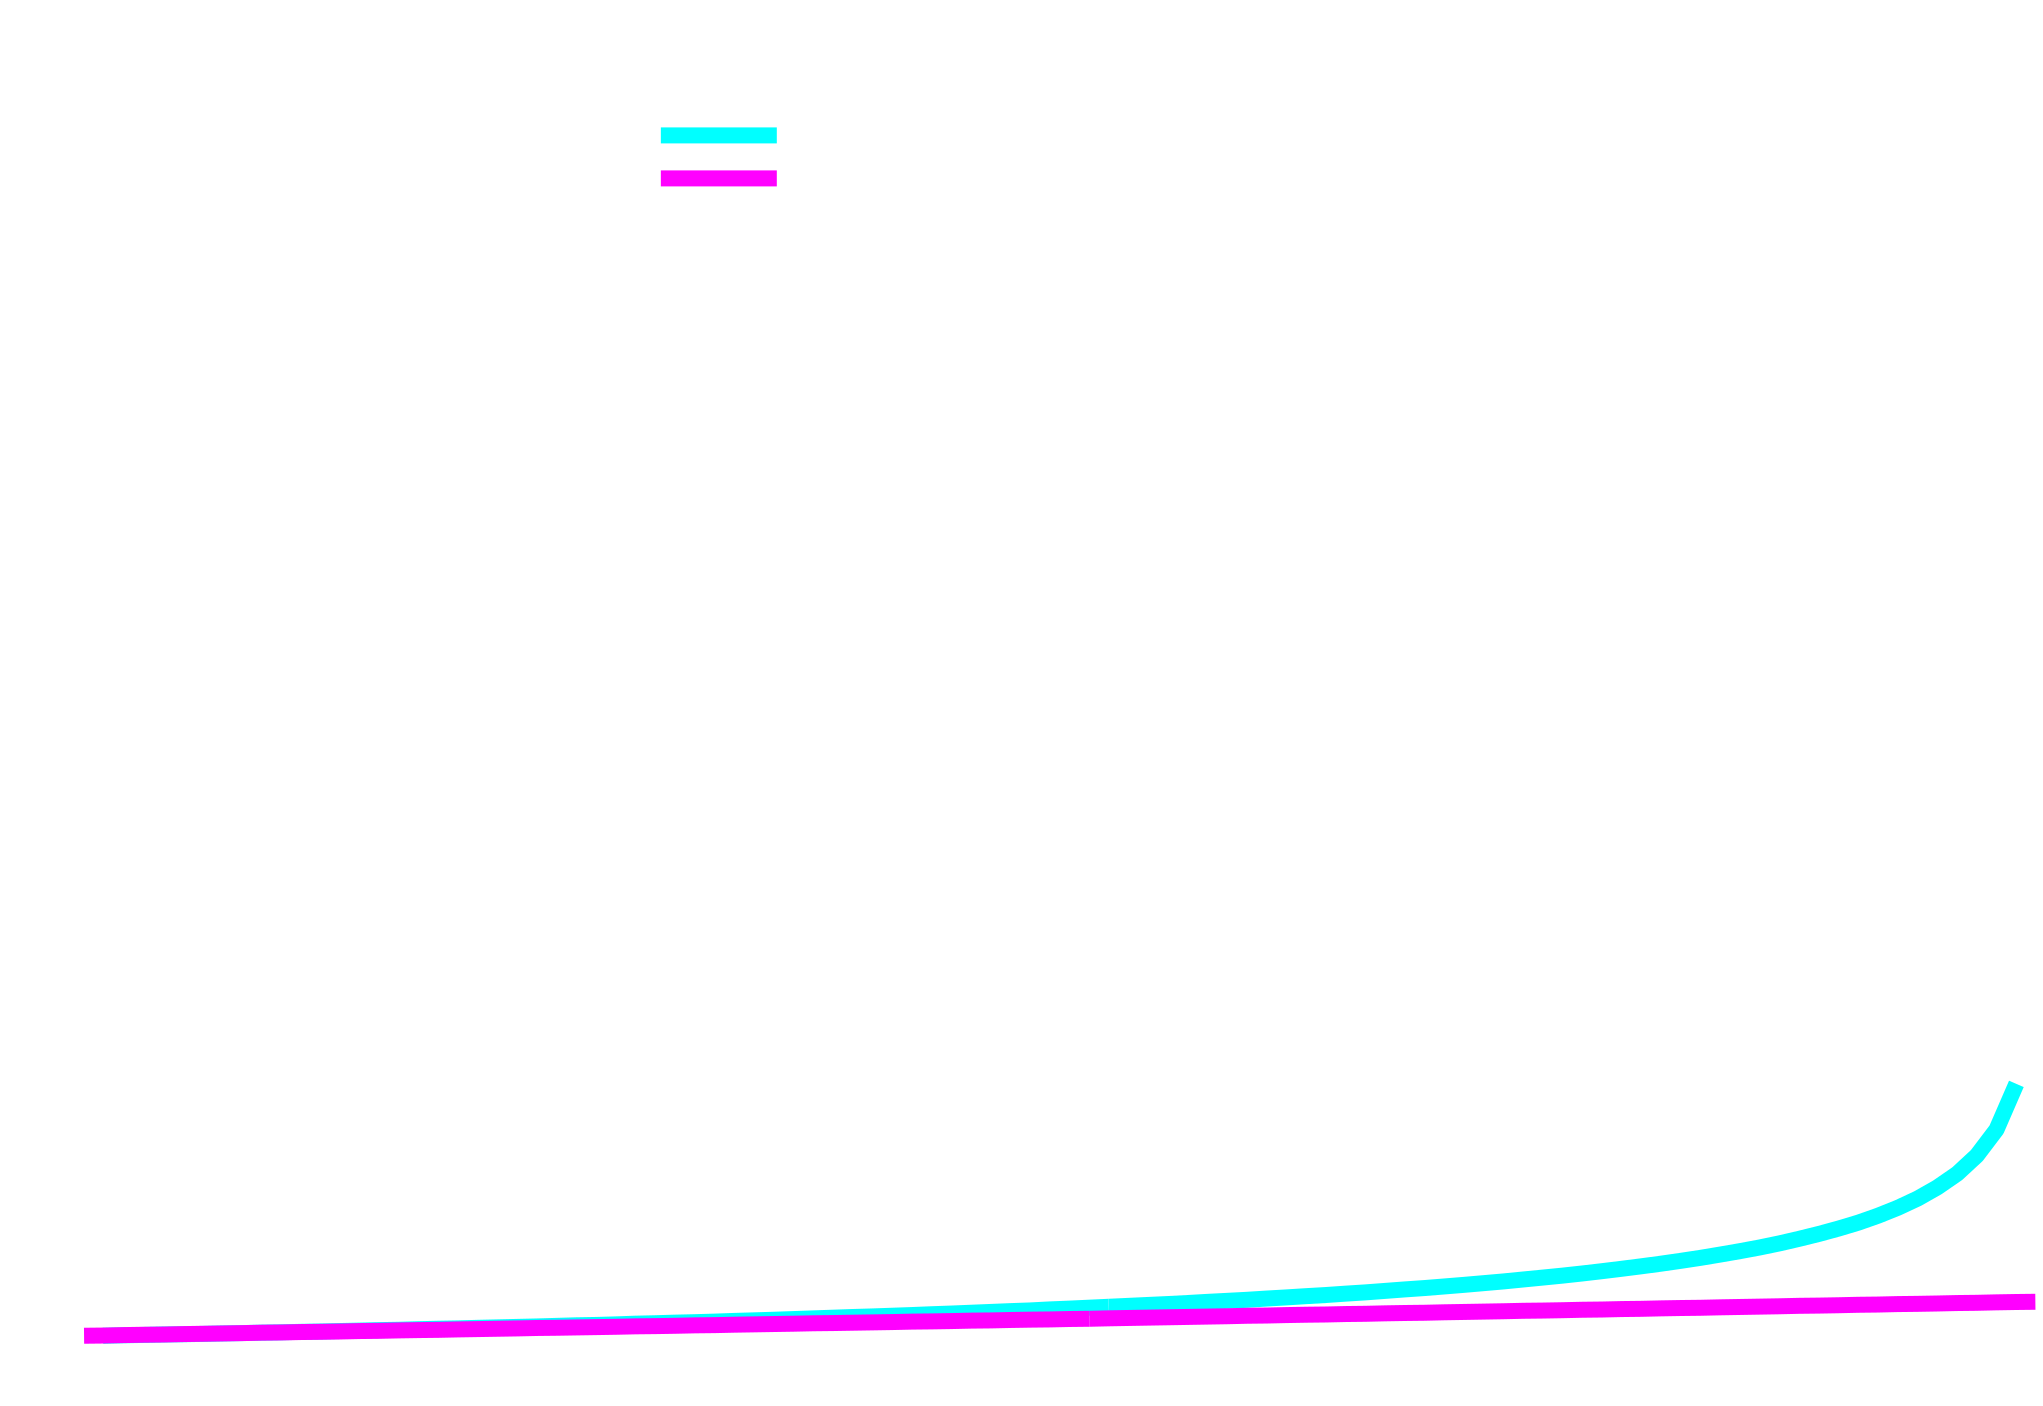
\includegraphics[width=0.667\textwidth]{probesByLoadFactor}%
    }\\
  & Load Factor\\
\end{tabular}
\end{figure}
\end{frame}

\begin{frame}{Probes in Unsuccessful Search}
\begin{figure}\centering
\begin{tabular}{rc}
    \rotatebox[origin=c]{90}{Average \# of Probes}
  &
    \raisebox{\dimexpr-.5\height}{
    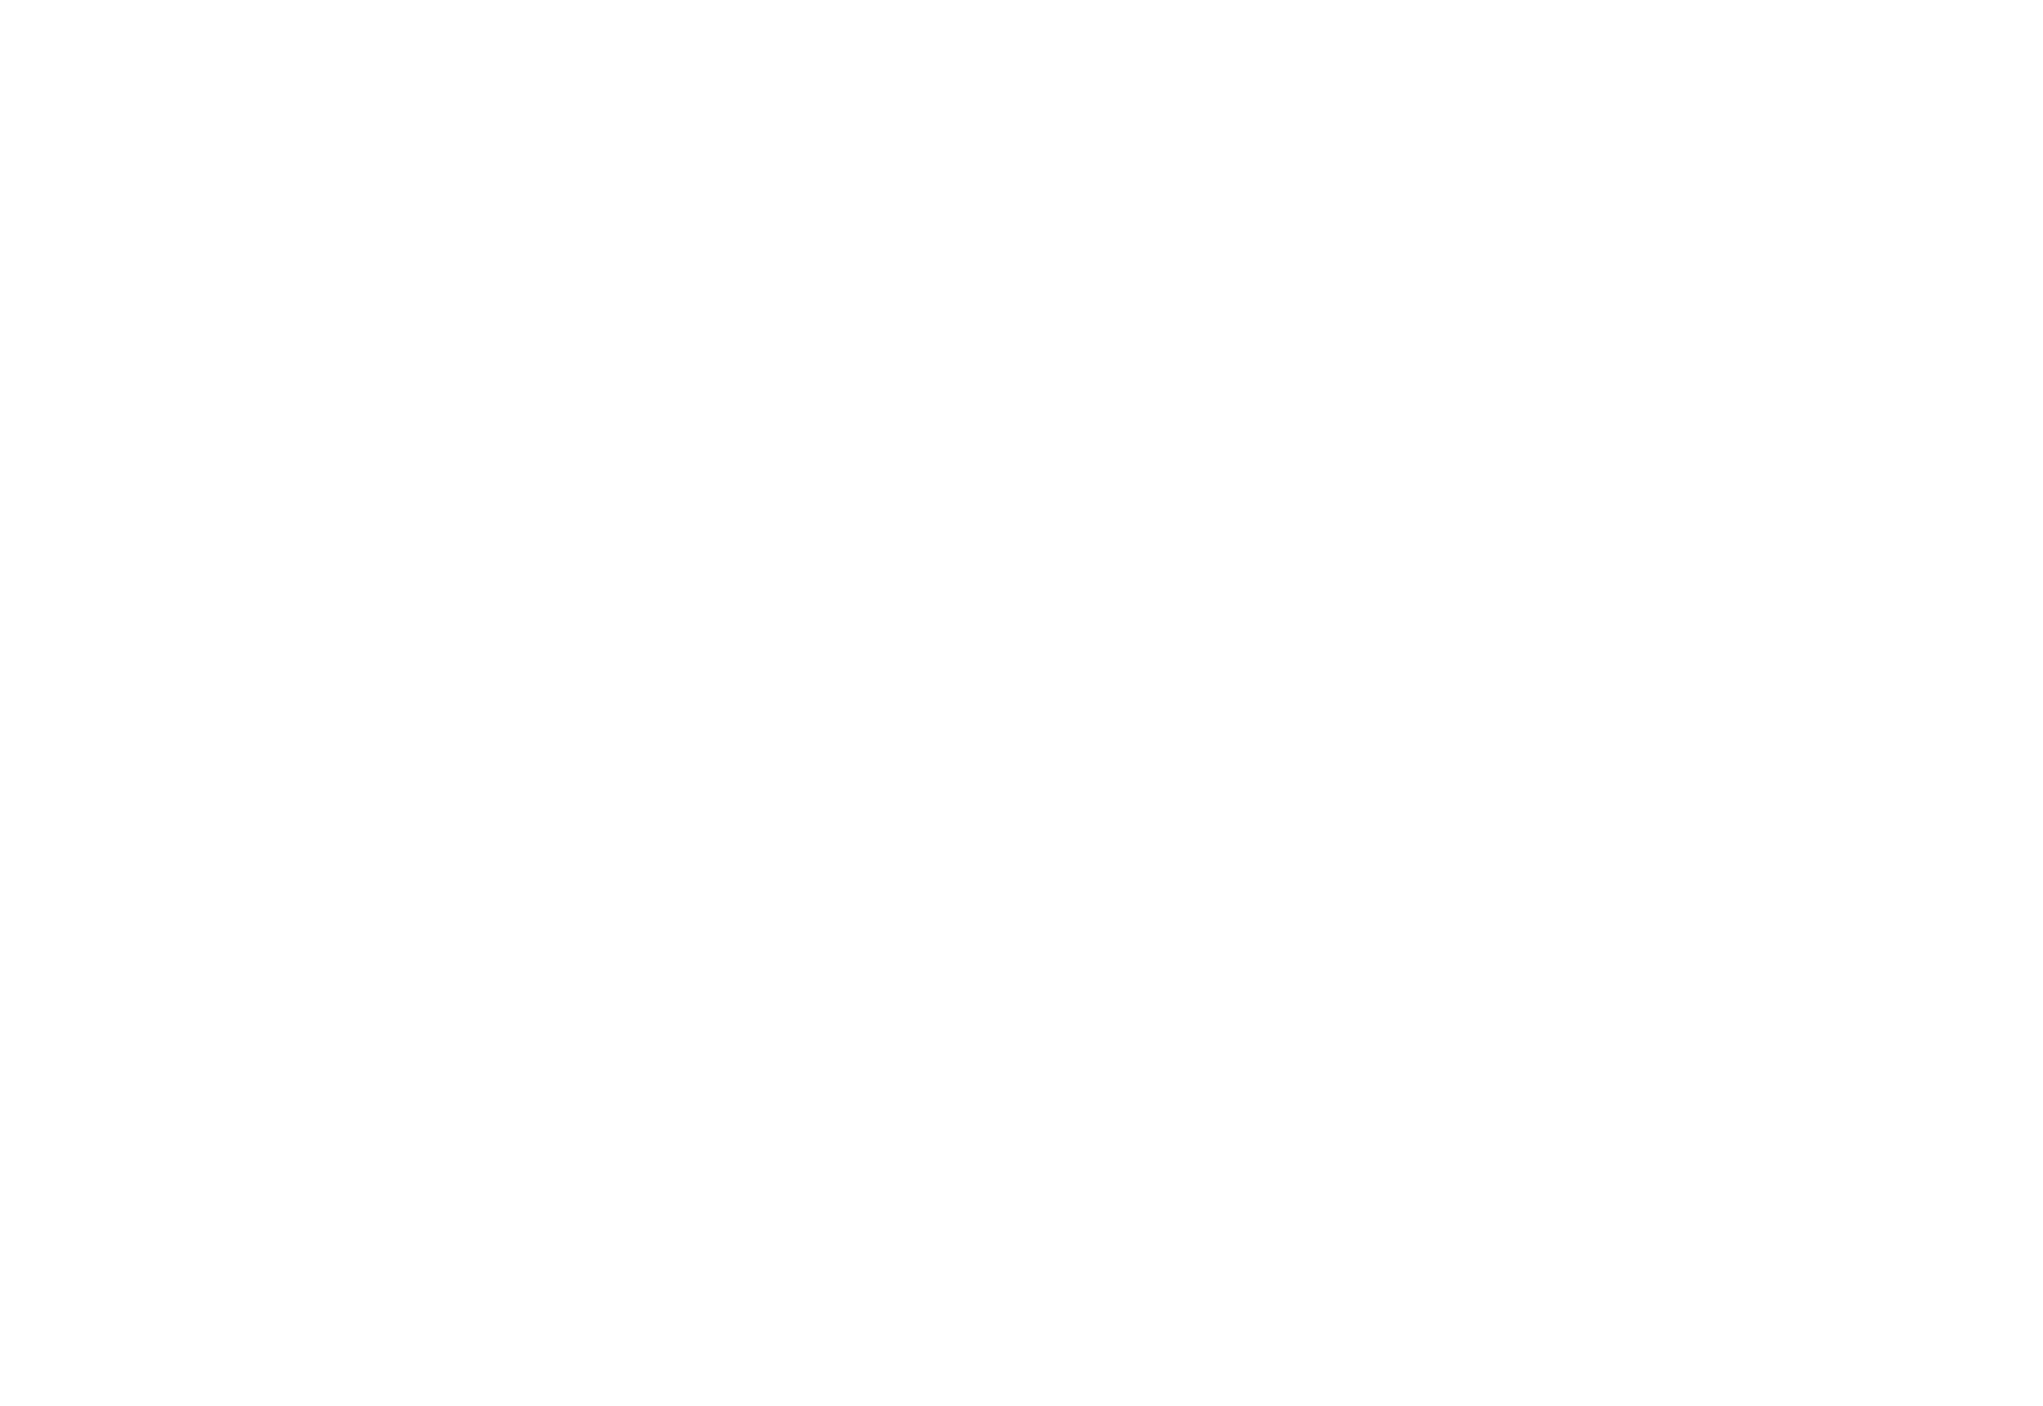
\includegraphics[width=0.667\textwidth]{probesUnsuccessfulByLoadFactor}%
    }\\
  & Load Factor\\
\end{tabular}
\end{figure}
\end{frame}

\begin{frame}{CPU Cache Misses Required for Look-Up}
\begin{columns}
\column{0.6\textwidth}
\begin{figure}\centering
\begin{tabular}{rc}
    \rotatebox[origin=c]{90}{\small Average cache misses per lookup}
  &
    \raisebox{\dimexpr-.5\height}{
    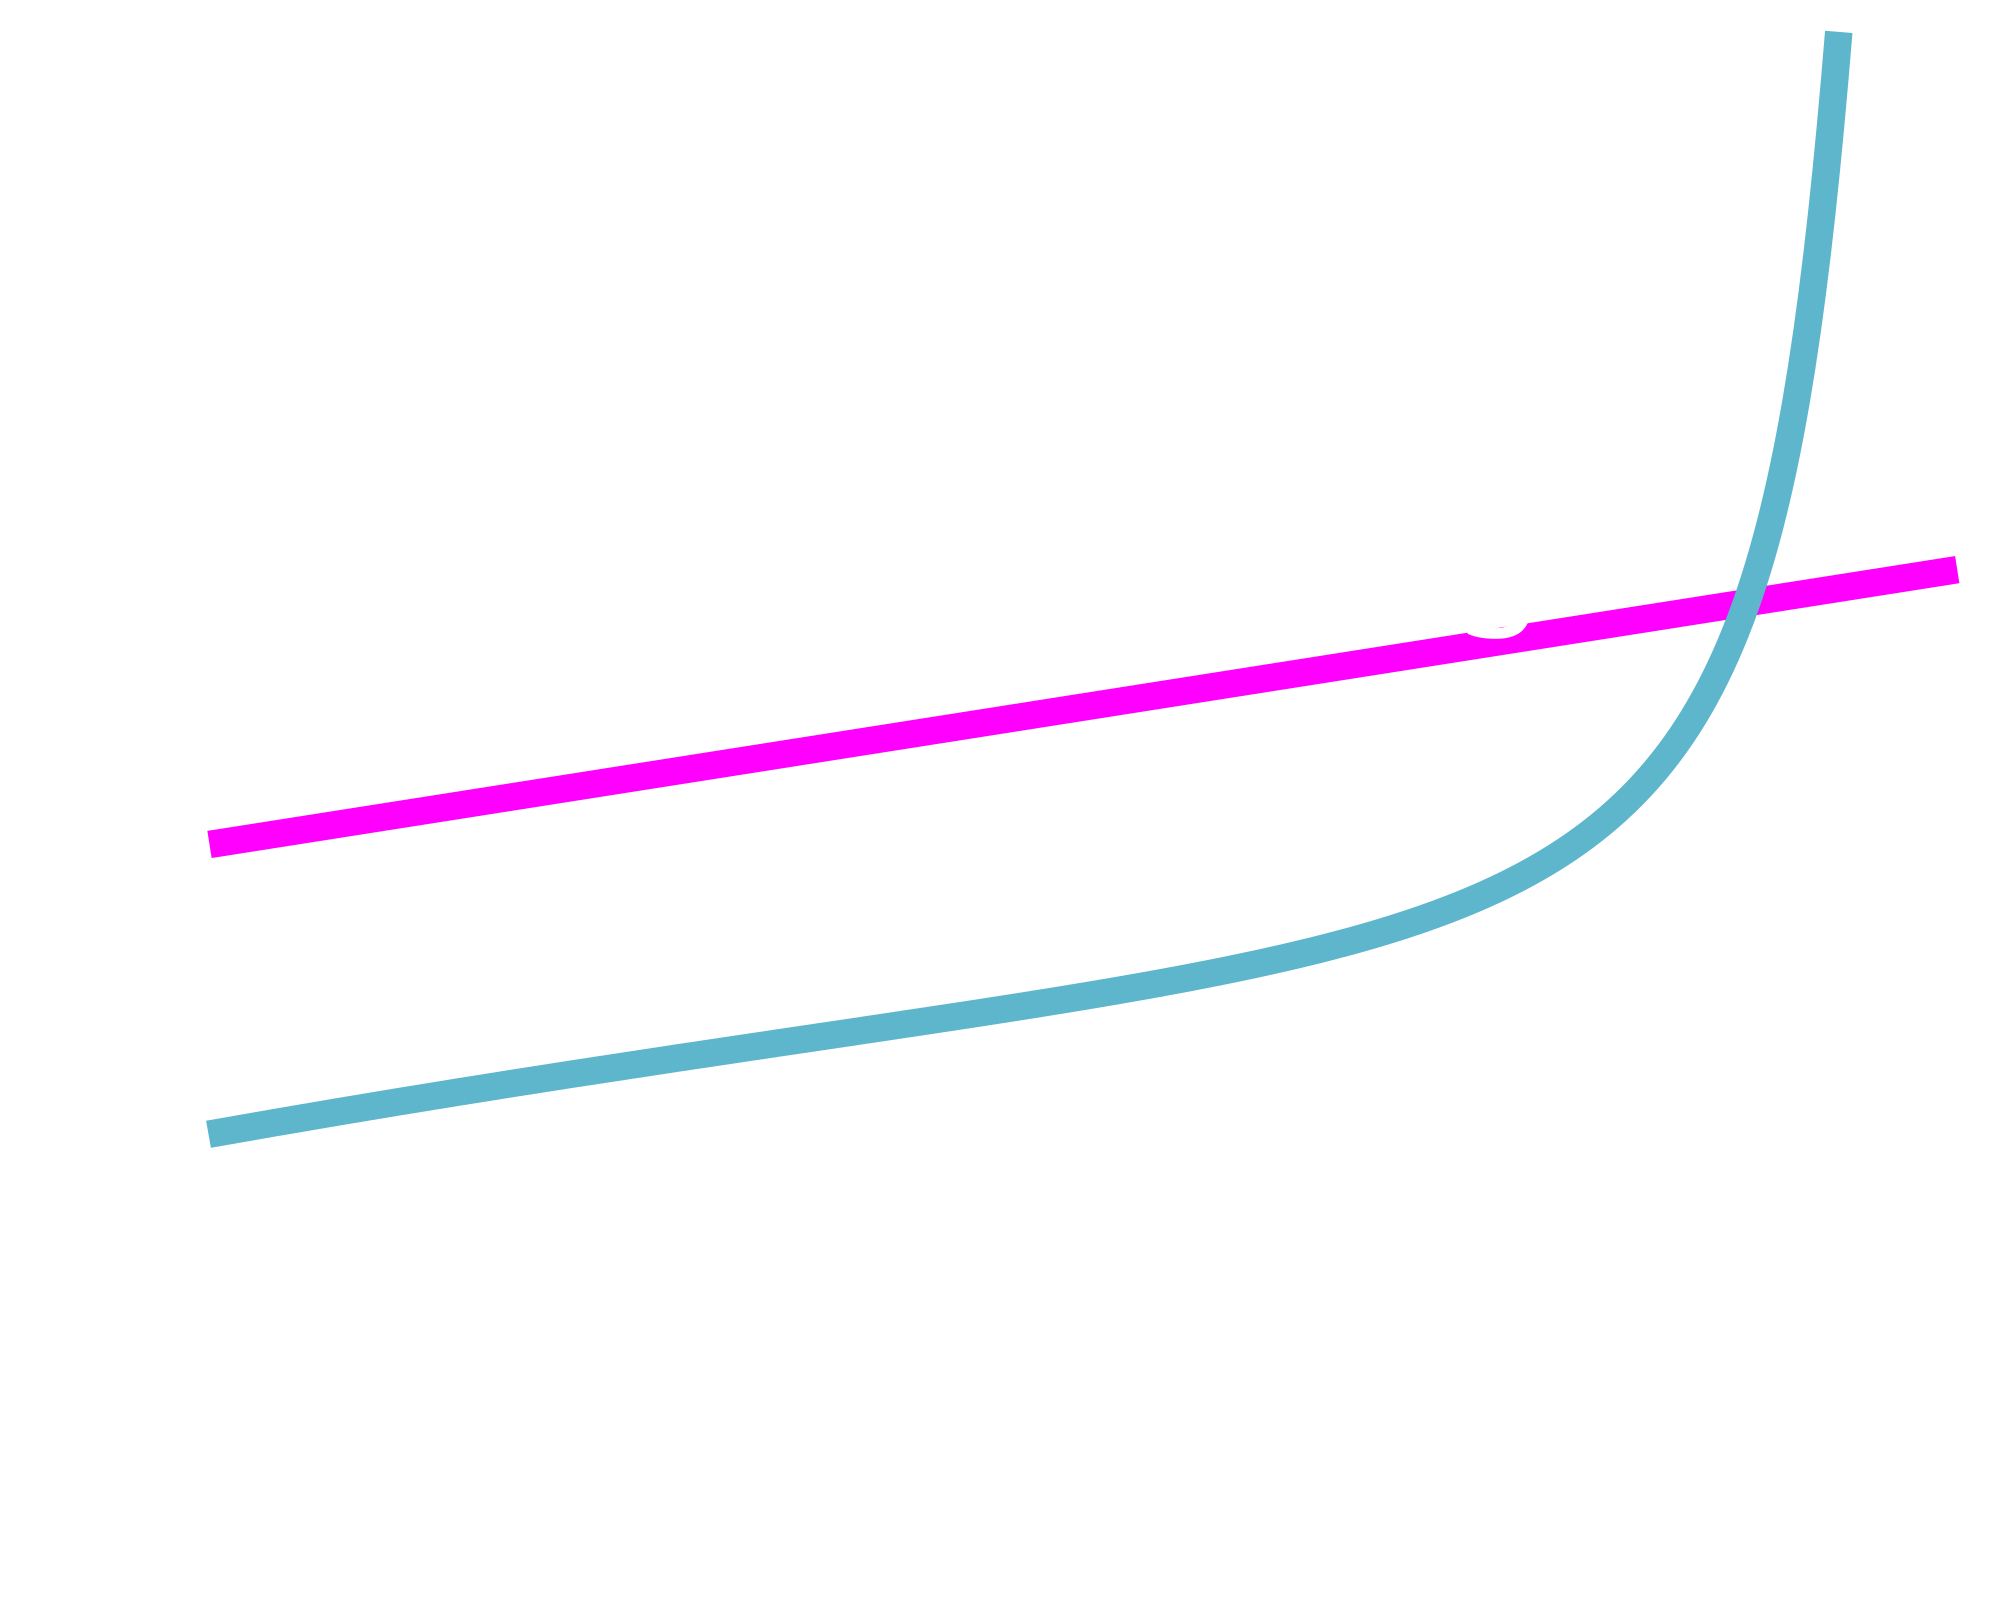
\includegraphics[width=0.85\textwidth]{probesCacheMisses}%
    }\\
  & {\small Load Factor}\\
\end{tabular}
\end{figure}
\column{0.4\textwidth}
In large hash tables that far exceed the CPU cache size, linear probing performs better due to better locality of reference. However, linear probing performs poorly as the table gets full.
\end{columns}
\end{frame}

\section{Deletion}
\begin{frame}{Deletion in Open Addressing}
% \begin{columns}[b]
% \column{0.3\textwidth}
\centerline{%
\begin{tikzpicture}[%
  node of array/.append style={%
    minimum height=8mm,
    inner sep=0,
    text depth=.1ex,
    minimum width=11mm,
    %fill=CSUslate,
    %text=white!50!CSUslate
  },%
  subcomponent of array el/.append style={minimum width=11mm, node distance=-1.4pt},%
  node distance=11pt%
]%
  \ArrayLabel{}
  
  \ArrayNodeVertical{0,\textellipsis}
  \node[block] (firstArrayEl) [fit=(val) (lastElValue)]{};
  \node (Above) [above=of $(val)!0.5!(lastElValue)$] {\alt<-2>{insert(7)}{\alt<-4>{delete(2)}{find(7)}}};
  % \node[anchor=south, text depth=.2ex, name=keyCol] at ([yshift=-1pt] val.north) {key};
  % \node[anchor=south, text depth=.2ex, name=keyCol] at ([yshift=-1pt] lastElValue.north) {value};


  \ArrayNodeVertical{1,\textellipsis}
  \alt<-3>{
    \ArrayNodeVertical{2,\textellipsis}
  }{
    \alt<-7>{
      \begin{scope}[node of array/.append style = {fill=CSUslate, text=white!50!CSUslate}]
        \ArrayNodeVertical{?,?}
      \end{scope}
    }{
      \begin{scope}[node of array/.append style = {fill=MyPurple, text=white!50!MyPurple}]
        \ArrayNodeVertical{2,\textellipsis}
      \end{scope}
    }
  }
  \onslide<6-7>{%
    % \node[anchor=west] (where) at ([xshift=0.5em, yshift=4mm] lastElValue.east) {Where is it?};
    \node (where) [right=of lastElValue.north east] {Where is it?};
    \draw[link, ->] (where) to[bend left=20] (prev);%
  }
  \alt<1>{
    \begin{scope}[node of array/.append style = {fill=CSUslate, text=white!50!CSUslate}]
      \ArrayNodeVertical{?,?}
    \end{scope}
  }{\ArrayNodeVertical{7,\textellipsis}}

  \begin{scope}[node of array/.append style = {fill=CSUslate, text=white!50!CSUslate}]
    \ArrayNodeVertical{?,?}
    \ArrayNodeVertical{?,?}
    \ArrayNodeVertical{?,?}
    % \node[block] (lastArrayEl) [fit=(val) (lastElValue)]{};
  \end{scope}

  \onslide<7->{%
    \node (RightNote) [right=of $(firstArrayEl.east)!0.5!(lastElValue.east)$, align=left, anchor=north west] {Must use lazy deletion!\\[0.5em]
    On insertion, treat a (lazily)\\ deleted item as an empty slot.};
  }
\end{tikzpicture}}%
\onslide<8>{}
% \column{0.5\textwidth}
% \onslide<7->{%
% Must use lazy deletion!

% On insertion, treat a (lazily) deleted item as an empty slot.\vspace{1em}}
% \end{columns}
\end{frame}

\section*{Method Comparison}
\begin{frame}{Open Addressing vs.Separate Chaining}
\begin{itemize}
  \item
    When should you be concerned about Open Addressing and Separate Chaining implementations?
  \item<-2>
    When implementing a hash table, consider:
    \begin{itemize}
      \item
        Do you know the number of items to be inserted into the table?
      \item
        Do you have plenty of memory?
      \item
        Do you know the expected load factor?
    \end{itemize}
\end{itemize}
\end{frame}

\begin{frame}{Hash Tables in the STL}

  \begin{tabular}{r  l  l}
    \toprule%
      & \textbf{No duplicates} & \textbf{Duplicates} \\
    \midrule%
      \textbf{Key-Only}
        & \href{https://en.cppreference.com/w/cpp/container/unordered_set}{{\small{}std::}unordered\_set}
        & \href{https://en.cppreference.com/w/cpp/container/unordered_multiset}{{\small{}std::}unordered\_multiset} \\
      \textbf{Key-Value Pair}
        & \href{https://en.cppreference.com/w/cpp/container/unordered_map}{{\small{}std::}unordered\_map}
        & \href{https://en.cppreference.com/w/cpp/container/unordered_multimap}{{\small{}std::}unordered\_multimap}\\
    \bottomrule%
  \end{tabular}
  \vspace{0.25em}

  \href{https://en.cppreference.com/w/cpp/utility/hash}{\texttt{std::hash}} is defines the default hash functions as function objects.
  \vspace{0.25em}
  
  * You may not use these containers for labs 18 and 19.
\end{frame}


\section*{Lab 19}
\begin{frame}{Lab 19: Hash Tables with Open Addressing}
\begin{center}\Large
Let's take a look at the lab based on today's lecture.
\end{center}
\end{frame}

\end{document}